\documentclass[a4paper,10pt,notitlepage]{report}
\usepackage[T1]{fontenc}
\usepackage[left=1in, right=1in, top=0.2in, bottom=0.0in]{geometry}
\usepackage{graphicx}

\usepackage{titling}
\usepackage{lipsum}

\graphicspath{ {.} }

\pretitle{\begin{center}\Large\bfseries}
\posttitle{\par\end{center}\vskip 0.5em}
\preauthor{\begin{center}\Large\ttfamily}
\postauthor{\end{center}}

\title{Programowanie współbieżne, zadanie 3 - Współbieżność w C++. Raport o wydajności}
\author{Karol Baryła kb406092}
\begin{document}
\date{}

\maketitle
\thispagestyle{empty}



\begin{section}*{Platforma testowa}
Test przeprowadziłem na 2 komputerach:\\
1. Serwer students: AMD Opteron(tm) Processor 6386 SE (16C/16T, 2.8-3.5GHz, L1 48KB, L2 16MB, L3 16MB), 128GB RAM.\\
2. Prywatny laptop: Intel(R) Core(TM) i7-7500U (2C/4T, 2.7-3.5GHz, L1 32KB D/32KB I, L2 2 x 256 KB, L3 4MB), 8GB RAM.\\
\end{section}

\begin{section}*{Problem plecakowy}
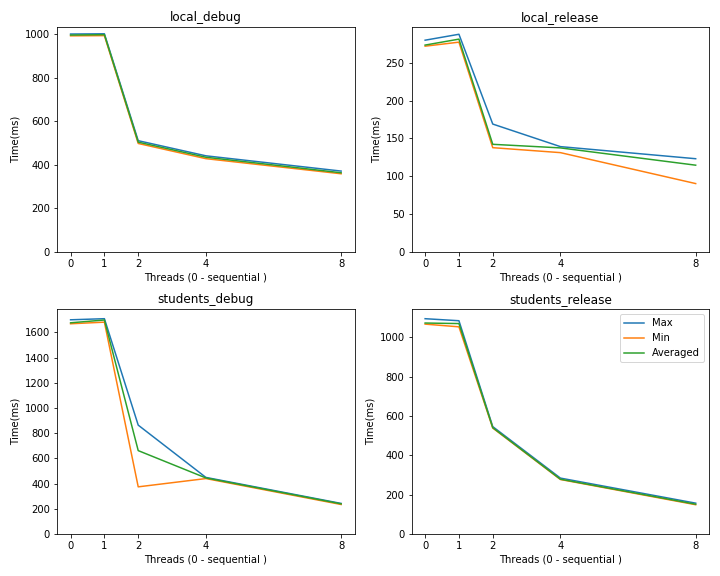
\includegraphics[width=12.5cm, height=10cm]{backpack.png}\\
To co warto zauważyć, to ogromną różnicę między trybami Debug i Release (na moim laptopie ~4-krotnie szybciej na Release). Oprócz tego - powyżej 2 wątków brak praktycznego przyśpieszenia na moim laptopie, mimo włączonego HT a więc 4 wątków wirtualnych. Na students skaluje się ładnie, chociaż nie idealnie liniowo.
\end{section}

\begin{section}*{Największy element}
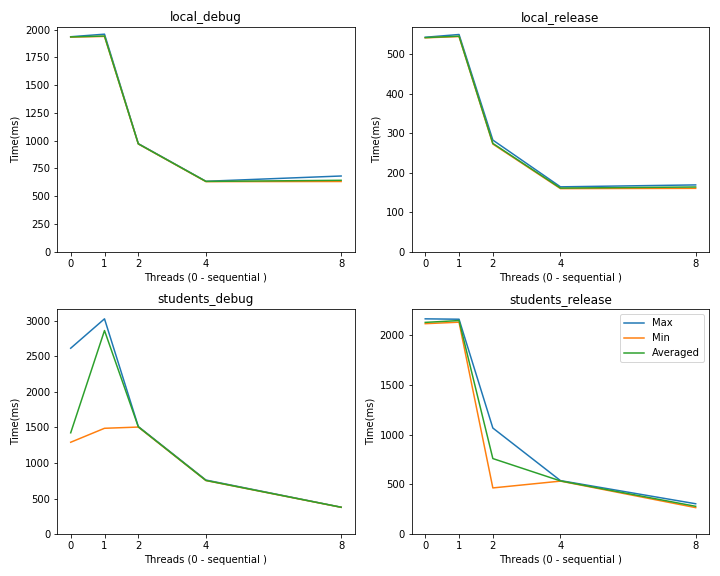
\includegraphics[width=12.5cm, height=10cm]{max.png}\\
Tym razem na moim laptopie skalowanie takie jak być powinno - do 4 wątków w miarę liniowo, potem brak. Na students wyniki bardzo rozbieżne (czyżby nagłe zmiany obciążenia serwera?), jednak śledząc wykres Max widać skalowanie aż do 8 wątków. Co ciekawe, przyspieszenie przy przejściu 1 wątek -> 2 wątki jest więcej niż dwukrotne. Dalej ogromna różnica między Debug a Release.
\end{section}

\begin{section}*{Merge sort}
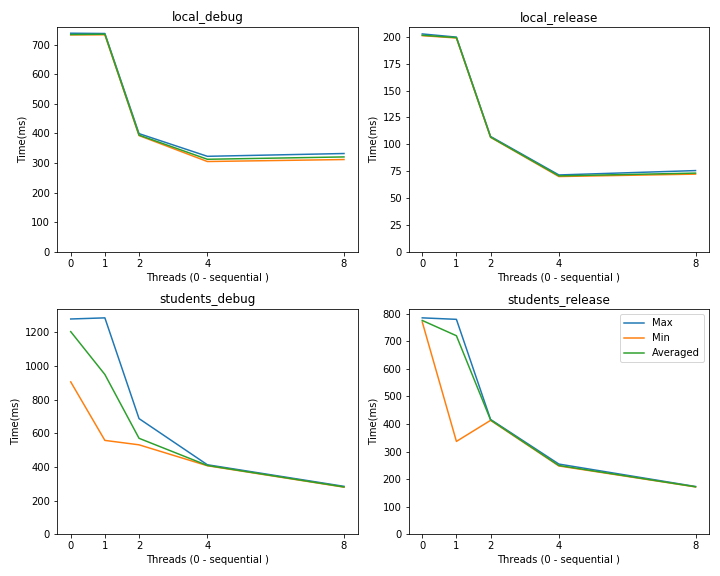
\includegraphics[width=12.5cm, height=10cm]{sort.png}\\
Bardzo podobnie jak wyżej - na moim laptopie wyniki przewidywalne, na students także, jednak czytelność wyników zaburza znaczny ich rozrzut przy mniejszej ilości wątków.
\end{section}

\end{document}
